%!TEX root =../../course-notes.tex
% ^ leave for LaTeXTools build functionality

\begin{module}{Module R: Euclidean Vector Space}

\begin{moduleStandards}
  \item \textbf{R1. Spanning Euclidan Space}
        Determine if a set of Euclidean vectors spans \(\IR^n\).
  \item \textbf{R3. Linear Independence.}
        Determine if a set of Euclidean vectors is linearly dependent or
        independent.
  \item \textbf{R4. Basis Verification}
        Determine if a set of Euclidean vectors is a basis for \(\IR^n\).
  \item \textbf{R5. Basis Computation}
        Compute a basis for a subspace of \(\IR^n\).
  \item \textbf{R6. Dimension}
        Compute the dimension for a subspace of \(\IR^n\).
\end{moduleStandards}

%!TEX root =../../course-notes.tex
% ^ leave for LaTeXTools build functionality

%!TEX root =../../course-notes.tex
% ^ leave for LaTeXTools build functionality


\begin{readinessAssuranceOutcomes}
\item Determine if a system to a two-variable system of linear equations
      will have zero, one, or infinitely-many solutions by graphing.
\item Find the unique solution to a two-variable system of linear equations
      by back-substitution.
\end{readinessAssuranceOutcomes}

\begin{readinessAssuranceResources}
\item \url{https://www.khanacademy.org/math/cc-eighth-grade-math/cc-8th-systems-topic/cc-8th-systems-graphically/a/systems-of-equations-with-graphing}
\item \url{https://www.khanacademy.org/math/algebra/systems-of-linear-equations/solving-systems-of-equations-with-substitution/v/practice-using-substitution-for-systems}
\end{readinessAssuranceResources}




\begin{readinessAssuranceTest}
\item Which of these graphs represents the following system of linear equations?
      \begin{align*}
      x+2y   &=   4 \\
      2x-3y  &=  1
      \end{align*}

\begin{multicols}{4}
\begin{readinessAssuranceTestChoices}
\item \systemWithOneSolutionA % correct
\item \systemWithOneSolutionB
\item \systemWithInfinitelyManySolutions
\item \systemWithNoSolutions
\end{readinessAssuranceTestChoices}
\end{multicols}

\item Which of these graphs represents the following system of linear equations?
      \begin{align*}
      3x+3y   &=   6 \\
      x+y  &=  2
      \end{align*}

\begin{multicols}{4}
\begin{readinessAssuranceTestChoices}
\item \systemWithOneSolutionA
\item \systemWithOneSolutionB
\item \systemWithInfinitelyManySolutions % correct
\item \systemWithNoSolutions
\end{readinessAssuranceTestChoices}
\end{multicols}


\item How many solutions are there for the system of linear equations
      represented by the following graph?
    \begin{center}
      \systemWithOneSolutionB
    \end{center}

\begin{multicols}{4}
\begin{readinessAssuranceTestChoices}
\item Zero
\item One % correct
\item Two
\item Infinitely-many
\end{readinessAssuranceTestChoices}
\end{multicols}


\item How many solutions are there for the system of linear equations
      represented by the following graph? (This graph represents two completely
      overlapping lines.)
    \begin{center}
      \systemWithInfinitelyManySolutions
    \end{center}

\begin{multicols}{4}
\begin{readinessAssuranceTestChoices}
\item Zero
\item One
\item Two
\item Infinitely-many % correct
\end{readinessAssuranceTestChoices}
\end{multicols}


\item How many solutions are there for the system of linear equations
      represented by the following graph?
    \begin{center}
      \systemWithOneSolutionA
    \end{center}

\begin{multicols}{4}
\begin{readinessAssuranceTestChoices}
\item Zero
\item One % correct
\item Two
\item Infinitely-many
\end{readinessAssuranceTestChoices}
\end{multicols}


\item How many solutions are there for the system of linear equations
      represented by the following graph? (This graph represents two
      non-overlapping parallel lines.)
    \begin{center}
      \systemWithNoSolutions
    \end{center}

\begin{multicols}{4}
\begin{readinessAssuranceTestChoices}
\item Zero % correct
\item One
\item Two
\item Infinitely-many
\end{readinessAssuranceTestChoices}
\end{multicols}

\item Solve the following system of linear equations.
      \begin{align*}
      y   &=   2x+5 \\
      y  &=  -x+2
      \end{align*}

\begin{multicols}{4}
\begin{readinessAssuranceTestChoices}
\item \((x,y)=(-1,3)\) % correct
\item \((x,y)=(4,-2)\)
\item There are no solutions.
\item There are infinitely-many solutions.
\end{readinessAssuranceTestChoices}
\end{multicols}

\item Solve the following system of linear equations.
      \begin{align*}
      y   &=  3x+5 \\
      y  &=  3x+2
      \end{align*}

\begin{multicols}{4}
\begin{readinessAssuranceTestChoices}
\item
\((x,y)=(3,4)\)
\item
\((x,y)=(-5,1)\)
\item There are no solutions. % correct
\item There are infinitely-many solutions.
\end{readinessAssuranceTestChoices}
\end{multicols}

\item Solve the following system of linear equations.
      \begin{align*}
      x+2y   &=   4 \\
      2x-3y  &=  1
      \end{align*}

\begin{multicols}{4}
\begin{readinessAssuranceTestChoices}
\item
\((x,y)=(-1,4)\)
\item
\((x,y)=(2,1)\) % correct
\item There are no solutions.
\item There are infinitely-many solutions.
\end{readinessAssuranceTestChoices}
\end{multicols}

\item Solve the following system of linear equations.
      \begin{align*}
      4x-8y   &= 12 \\
      -6x+12y  &=  18
      \end{align*}

\begin{multicols}{4}
\begin{readinessAssuranceTestChoices}
\item
\((x,y)=(3,3)\)
\item
\((x,y)=(-2,1)\)
\item There are no solutions.
\item There are infinitely-many solutions. % correct
\end{readinessAssuranceTestChoices}
\end{multicols}

\end{readinessAssuranceTest}

%!TEX root =../../course-notes.tex
% ^ leave for LaTeXTools build functionality

\begin{applicationActivities}{Day 1}

\begin{activity}{10}
  How many vectors are required to span \(\IR^2\)?
  Sketch a drawing in the \(xy\) plane to support your guess.
\end{activity}

\begin{fact}
  At least \(n\) vectors are required to span \(\IR^n\).

  \begin{center}
  \begin{tikzpicture}[scale=0.5]
    \draw[<->] (-4,0) -- (4,0);
    \draw[<->] (0,-4) -- (0,4);
    \draw[blue!50] (2,-4) -- (-2,4);
    \draw[thick,blue,->] (0,0) -- (1,-2);
  \end{tikzpicture}
  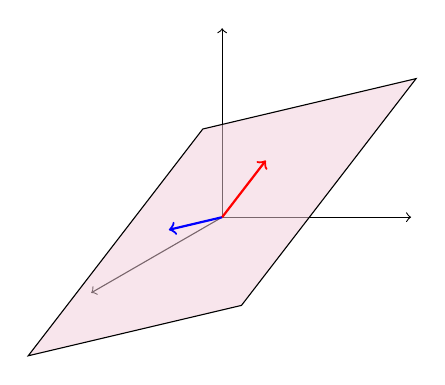
\begin{tikzpicture}[x={(210:0.8cm)}, y={(0:1cm)}, z={(90:1cm)},scale=0.4]
    \draw[->] (0,0,0) -- (6,0,0);
    \draw[->] (0,0,0) -- (0,6,0);
    \draw[->] (0,0,0) -- (0,0,6);
    \draw[fill=purple!20,fill opacity=0.5]
      (-2,-2,2) -- (6,-2,-2) -- (2,2,-2) -- (-6,2,2) -- (-2,-2,2);
    \draw[thick,blue,->] (0,0,0) -- (1,-1,0);
    \draw[thick,red,->] (0,0,0) -- (-2,0,1);
  \end{tikzpicture}
  \end{center}
\end{fact}

\begin{activity}{15}
  Find a vector \(\begin{bmatrix}a\\b\\c\end{bmatrix}\)
  in \(\IR^3\) that is not in
  \(\vspan\left\{\begin{bmatrix}1\\-1\\0\end{bmatrix},
  \begin{bmatrix}-2\\0\\1\end{bmatrix}\right\}\) by doing the following.
    \begin{subactivity}
      Choose simple values for \(x,y,z\) such that
      \(\begin{bmatrix}[cc|c]1&0&x\\0&1&y\\0&0&z\end{bmatrix}\)
      represents an inconsistent linear equation.
    \end{subactivity}
    \begin{subactivity}
      Use row operations to manipulate
      \(\begin{bmatrix}[cc|c]1&0&0\\0&1&0\\0&0&1\end{bmatrix}\sim
      \begin{bmatrix}[cc|c]1&-2&a\\-1&0&b\\0&1&c\end{bmatrix}\).
    \end{subactivity}
    \begin{subactivity}
      Write a sentence explaining why \(\begin{bmatrix}a\\b\\c\end{bmatrix}\)
      cannot be in \(\vspan\left\{\begin{bmatrix}1\\-1\\0\end{bmatrix},
      \begin{bmatrix}-2\\0\\1\end{bmatrix}\right\}\).
    \end{subactivity}
\end{activity}

\begin{fact}
  The set \(\{\vect v_1,\dots,\vect v_m\}\) fails to span all of \(\IR^n\)
  exactly when \(\RREF[\vect v_1\,\dots\,\vect v_m]\) has a row of zeros.
\end{fact}

\begin{activity}{10}
  Consider the set of vectors \(S=\left\{
  \begin{bmatrix}2\\3\\0\\-1\end{bmatrix},
  \begin{bmatrix}1\\-4\\3\\0\end{bmatrix},
  \begin{bmatrix}2\\0\\0\\3\end{bmatrix},
  \begin{bmatrix}0\\3\\5\\7\end{bmatrix},
  \begin{bmatrix}3\\13\\7\\16\end{bmatrix}
  \right\}
  \).
  \begin{subactivity}
  Prove that
  \(\IR^4=\vspan S\).
  \end{subactivity}
  \begin{subactivity}
  Find a linear combination of vectors in \(S\) that equals
  \(\begin{bmatrix}-1\\10\\7\\14\end{bmatrix}\).
  \end{subactivity}
\end{activity}

\begin{activity}{15}
  Consider the set of vectors \(S=\left\{
  \begin{bmatrix}2\\3\\0\\-1\end{bmatrix},
  \begin{bmatrix}2\\0\\0\\3\end{bmatrix},
  \begin{bmatrix}3\\13\\7\\16\end{bmatrix},
  \begin{bmatrix}-1\\10\\7\\14\end{bmatrix},
  \begin{bmatrix}4\\3\\0\\2\end{bmatrix}
  \right\}
  \).
  \begin{subactivity}
  Prove that
  \(\IR^4\not=\vspan S\).
  \end{subactivity}
  \begin{subactivity}
  Find a vector in \(\IR^4\) that is not in \(\vspan S\).
  \end{subactivity}
\end{activity}



\end{applicationActivities}


\end{module}
